\section{Projektmanagement}
Das Modul PREN ist ein interdisziplinäres Modul. Von jeder der Fachrichtungen Informatik, Elektrotechnik und Maschinenbau ist mindestens eine Person pro Gruppe vertreten. Das Team 27 setzt sich wie folgt zusammen:
\begin{itemize}
	\item 3 Informatiker
	\item 3 Maschinenbauer
	\item 1 Elektrotechniker
\end{itemize}
Zu Beginn des Moduls wurden den Mitgliedern des Teams verschiedene Funktionen zugewiesen, um eine Struktur und somit Ansprechpersonen innerhalb des Teams zu erhalten. Ersichtlich ist dies in folgendem Organigramm:
\begin{figure}[h!]
	\centering
	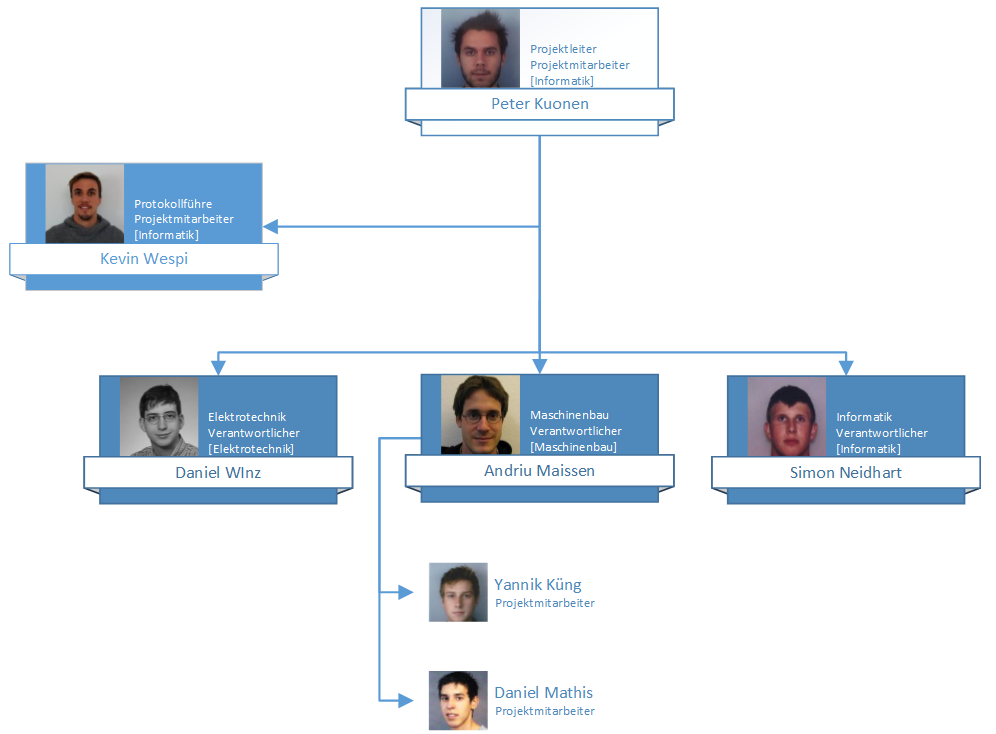
\includegraphics[width=0.7\textwidth]{fig/Organigramm.png}
	\caption{Organigramm}
	\label{fig:Organigramm}
\end{figure}

\subsection{Projektplanung}
In den folgenden Abbildungen wird die Planung mittels Zeitachsen für die einzelnen Meilensteine dargestellt. Sie enthalten die Hauptaufgaben, welche für die jeweiligen Meilensteine notwendig sind. Die Planung wurde angefertigt um die Übersicht über das Projekt zu haben und die verlangten Dokumente und Schritte zur Erfüllung der Meilensteine fristgerecht zu erledigen.

\begin{figure}[h!]
	\centering
	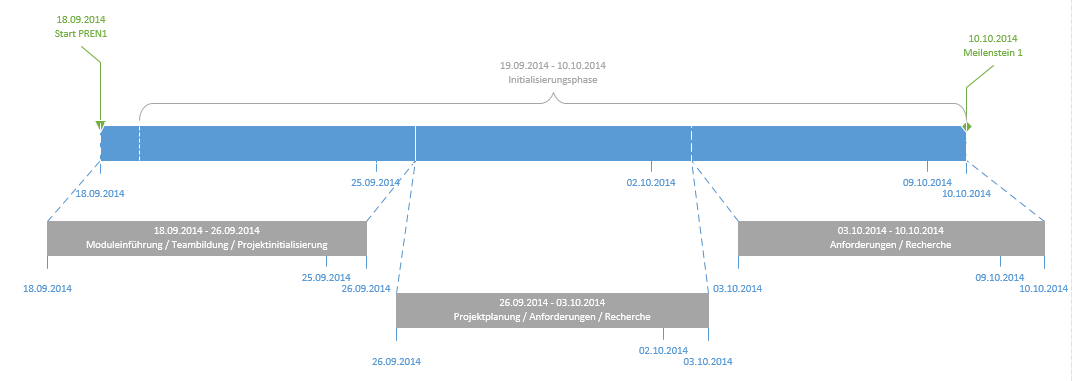
\includegraphics[angle=90,height=0.9\textheight]{fig/PlanungBisMS1.png}
	\caption{Planung Meilenstein 1}
	\label{fig:MS1}
\end{figure}
\begin{figure}[h!]
	\centering
	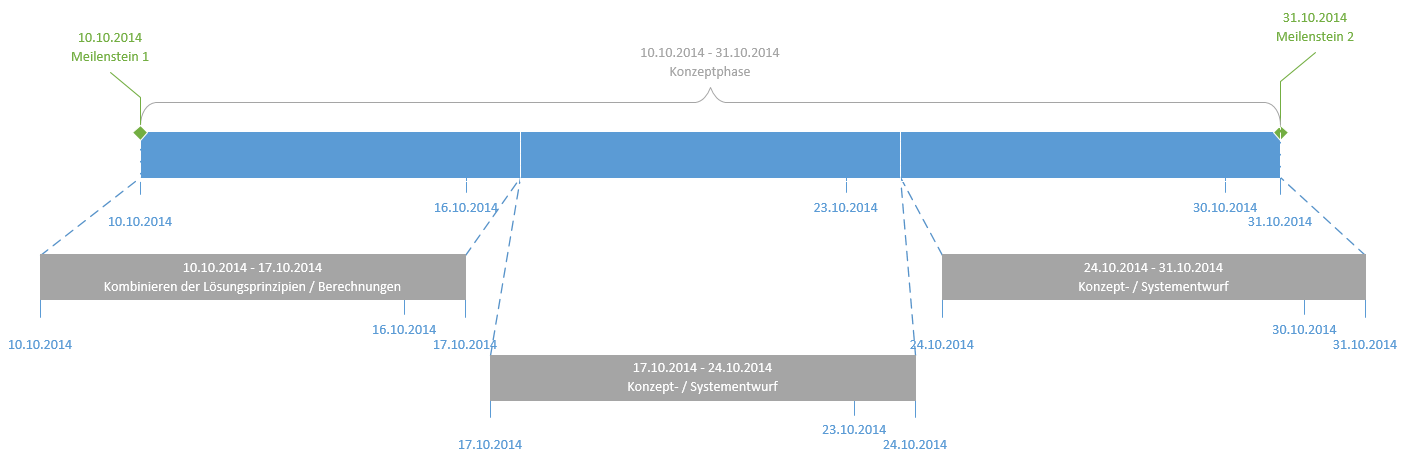
\includegraphics[angle=90,height=0.9\textheight]{fig/PlanungBisMS2.png}
	\caption{Planung Meilenstein 2}
	\label{fig:MS2}
\end{figure}
\begin{figure}[h!]
	\centering
	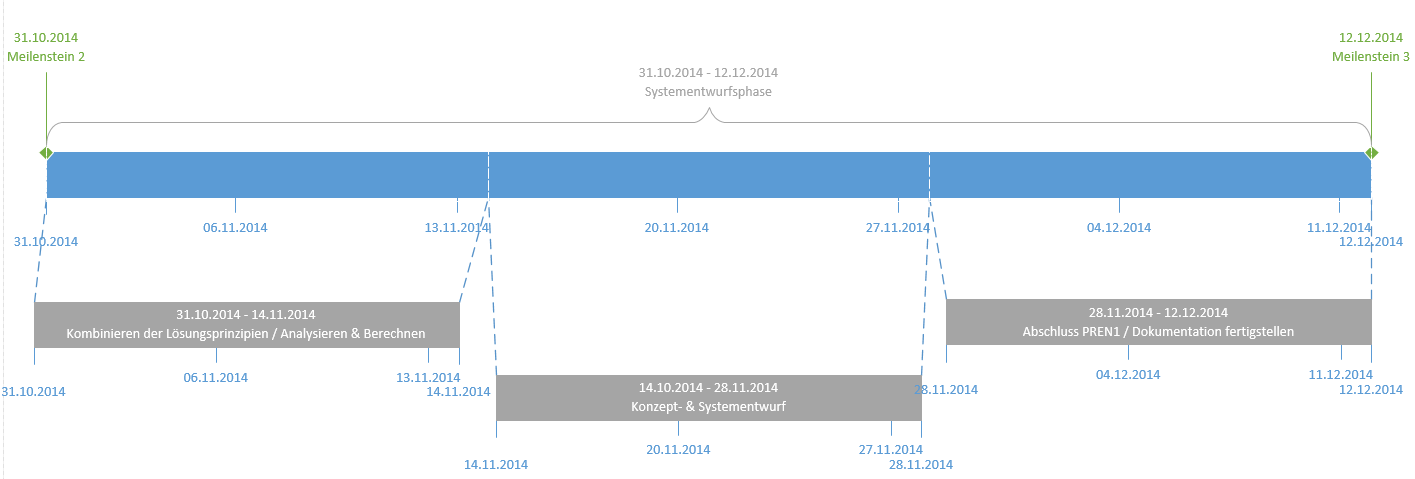
\includegraphics[angle=90,height=0.9\textheight]{fig/PlanungBisMS3.png}
	\caption{Planung Meilenstein 3}
	\label{fig:MS3}
\end{figure}
